\documentclass{beamer}

\usetheme{Berlin}

\usepackage{fontspec}
\usepackage{polyglossia}
\setmainlanguage{czech}

\usepackage{graphicx}
\usepackage{epstopdf}

\setlength{\unitlength}{0.5cm}

\title{Simulace SMP}
\author{Zdeněk Janeček \& Tomáš Cigler \& David Fiedler} 
\date{18.\,prosince 2015}

\begin{document}

\begin{frame} 
\titlepage
\end{frame}

\begin{frame} 
\frametitle{Zadání a úvod}
Vytvořte simulátor čtyřjádrového SMP a k němu:

\begin{itemize}
\item plánovač
\item synchronizaci procesů (semafory)
\item úlohu producent-konzument (poběží v osmi instancích)
\end{itemize}

\end{frame}


\begin{frame} 
\frametitle{Návrh implementace}

\begin{itemize}
\item AHoj!!
\end{itemize}


\end{frame}

\begin{frame} 
\frametitle{Rozhraní}

\end{frame}

\begin{frame} 
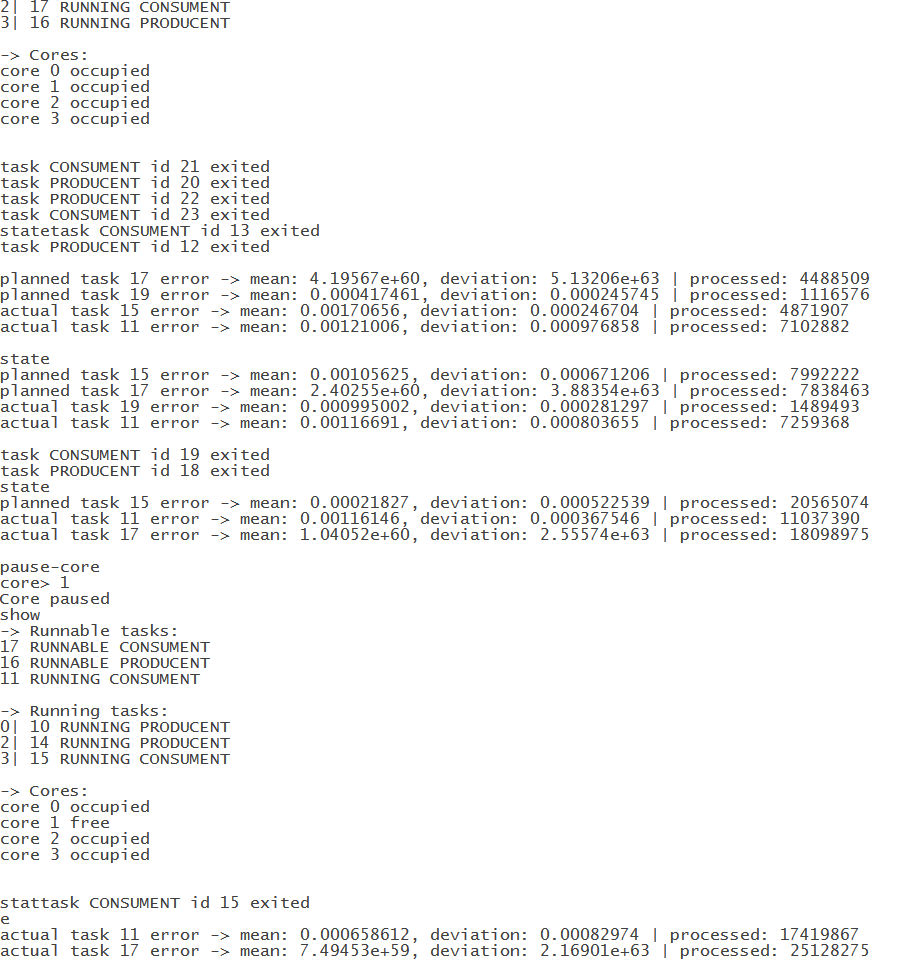
\includegraphics[height=\textheight]{obrazky/screen.png}

\end{frame}

\begin{frame} %[fragile]
\frametitle{Procesor - přerušení}

\end{frame}

\begin{frame} %[fragile]
\frametitle{Plánovač}

\end{frame}

\begin{frame} %[fragile]
\frametitle{Úlohy}

\end{frame}

\begin{frame} 
\frametitle{Výsledky a závěr}

\end{frame}

\end{document}
